\chapter{Test opracowanej biblioteki}
\label{cha:walidacja}

Zweryfikowane zostały trzy aspekty:

\begin{itemize}
\item poprawność zaprojektowania interfejsu programistycznego stworzonej biblioteki,
\item możliwość poprawnego nawiązania połączenia i przesłania danych między dwoma węzłami,
\item poprawność implementacji algorytmów kryptograficznych.
\end{itemize}

\section{Poprawność interfejsu programistycznego}

Poprawny interfejs programistyczny biblioteki musi umożliwiać implementację pełnego rozwiązania zapewniającego bezpieczną komunikację. Zostało to zweryfikowane poprzez stworzenie przykładowego oprogramowania wykorzystującego bibliotekę. Oprogramowanie to powstało na platformę Arduino oraz wykorzystuje moduł Bluetooth XM-15B do komunikacji.

Po uruchomieniu urządzenia inicjalizowana jest stworzona biblioteka implementujące bezpieczną komunikację, a moduł Bluetooth zostaje skonfigurowany w trybie \emph{slave} z nazwą ,,seconn'' i oczekuje na połączenie. Argumentami funkcji inicjalizującej bibliotekę są wskaźniki na następujące funkcje zaimplementowane w przykładowym oprogramowaniu:

\begin{itemize}
    \item funkcja obsługująca przekazywanie danych z biblioteki do modułu Bluetooth celem przesłania do drugiego węzła,
    \item funkcja obsługująca i przekazująca połączeniem szeregowym dane przychodzące z biblioteki, które zostały przez bibliotekę poprawnie uwierzytelnione oraz zdeszyfrowane,
    \item funkcja obsługująca powiadomienia o zmianie stanu połączenia przychodzące z biblioteki i przekazująca połączeniem szeregowym uwierzytelniony klucz publiczny drugiego węzła po nawiązaniu bezpiecznego połączenia,
    \item funkcja generująca liczby losowe stworzona w oparciu o implementację zaproponowaną w bibliotece {\itshape micro-ecc} (opis w dodateku~\ref{app:randgen}).
\end{itemize}

Dodatkowo zaimplementowane zostało przekazywanie połączeniem szeregowym klucza publicznego urządzenia celem weryfikacji z drugim węzłem oraz przekazywanie danych przychodzących z modułu Bluetooth do biblioteki. Przepływ danych między przykładowym oprogramowaniem, biblioteką, drugim węzłem oraz połączeniem szeregowym przedstawiono w Dodatku~\ref{app:samplediagram}.

Należy zwrócić uwagę, że oprogramowanie korzystające z biblioteki nie implementuje żadnej logiki związanej z protokołem komunikacji. Jest ona w całości zaimplementowana w bibliotece, a oprogramowanie jedynie zajmuje się przekazywaniem danych między fizycznym połączeniem a biblioteką. Całość oprogramowania wraz z funkcją generującą liczby losowe składa się ze 103 linii kodu, ośmiu funkcji i trzech plików.

W tabeli \ref{tab:sample-comm} przedstawiono przykładowe dane, jakie zostają przesłane przez połączenie szeregowe. W tym przypadku drugi węzeł był odpowiedzialny za rozpoczęcie połączenia (przesłanie pierwszego HelloRequest), a po poprawnym uwierzytelnieniu przesłał uwierzytelnioną i zaszyfrowaną wiadomość o treści ,,Some message...''.

\begin{table}
\centering
\caption{Przykładowe dane przesłane przez połączenie szeregowe. Stan nr 4 oznacza, że odebrany został prawidłowo uwierzytelniony pakiet HelloResponse zawierający klucz publiczny drugiego węzła.}
\begin{BVerbatim}
S!
Our pubkey is: 0x6D35D8BE2F0C67210C143E649F250FC4E
B014F25C305AC7C2FA6B02F0B4A4E63EA0BB52367AAF96E63B
BD968C186830ADE2B2A24769CB32E1E1A690F51079C7E
State:4
Pubkey of other side is: 0x22743237010F6830994886B
BFB781184C10D25E1D6819D075F40CF0724FEC049FF4804F82
58C14049E373595BC0987061B93493E16C8C59E8C7C2A64FF5
247B0
D:>Some message...<
\end{BVerbatim}
\label{tab:sample-comm}
\end{table}

\section{Poprawność implementacji algorytmów kryptograficznych}

Poprawność implementacji algorytmów CBC i dopełniania według PKCS\#7 stworzonych w ramach pracy oraz algorytmów AES, SHA-256 oraz ECDH dostarczonych przez zewnętrzne biblioteki została zweryfikowana poprzez stworzenie drugiej implementacji protokołu w języku Java.

Implementacje algorytmów AES, CBC, dopełniania według PKCS\#7, SHA-256 oraz ECDH pochodzą z pakietów java.security oraz javax.crypto biblioteki standardowej języka Java. Implementacja ECBC-MAC została wykonana w ramach pracy w oparciu o implementację CBC dostarczoną przez bibliotekę standardową. Użyte konfiguracje szyfrów to \emph{AES/CBC/NoPadding} i \emph{AES/ECB/NoPadding} do obliczania sygnatury oraz \emph{AES/CBC/PKCS7Padding} do szyfrowania i deszyfrowania.

W oparciu o tak stworzoną bibliotekę w języku Java napisano przykładową aplikację na platformę Android. Aplikacja po uruchomieniu stara się nawiązać połączenie Bluetooth z urządzeniem o nazwie ,,seconn''. Po nawiązaniu połączenia Bluetooth wywoływana jest metoda biblioteki służąca nawiązaniu bezpiecznego połączenia (wysłaniu pierwszego HelloRequest). Wszystkie zmiany stanu połączenia są na bieżąco wyświetlane na ekranie, a po nawiązaniu bezpiecznego połączenia wyświetlane są klucze publiczne obu węzłów i możliwe jest przesyłanie uwierzytelnionych i zaszyfrowanych danych do drugiego węzła.

Przykładowa aplikacja mobilna skutecznie połączyła się z urządzeniem AVR, a przesyłane dane były prawidłowo deszyfrowane, co potwierdza że implementacja algorytmów z zewnętrzych bibliotek AVR oraz implementacje wykonane w ramach pracy są zgodne z referencyjnymi implementacjami dostępnymi w bibliotece standardowej języka Java na platformie Android. Zrzut ekranu z aplikacji przedstawiono na rysunku \ref{fig:android}.

\begin{figure}
\centering
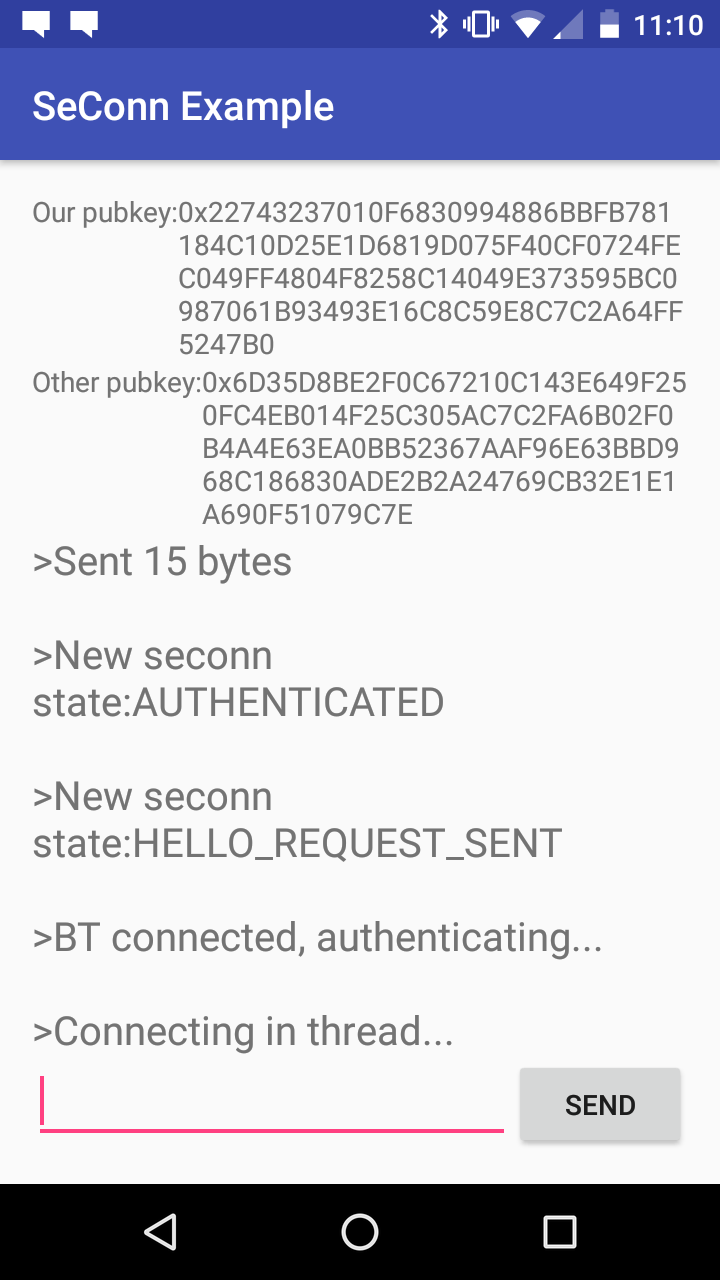
\includegraphics[height=0.6\textheight]{images/android.png}
\caption{Zrzut ekranu z przykładowej aplikacji implementującej protokół na platformę Android}
\label{fig:android}
\end{figure}
